\documentclass{alex_hü}

\name{Alexander Helbok}
\course{PS Physik}
\hwnumber{9}

\begin{document}
\renewcommand{\labelenumi}{\alph{enumi})}


\section*{132. Freier Fall einer rotierenden Hantel}
\begin{align*}
	m_1 &= 1 \unit{\kg};\quad &\vec{v}_1 &= \left(4, 0, 0\right) \unit{\m\per\s};\quad &\vec{r}_1 &= \left(0, 0, 2.5\right)\unit{\m}  \\
	m_2 &= 0.5 \unit{\kg};\quad  &\vec{v}_2 &= \left(1, 0, 0\right)\unit{\m\per\s};\quad &\vec{r}_2 &= \left(0, 0, 2.2\right)\unit{\m} 
\end{align*}
	\centering \( \vec{r}_{sp} = \dfrac{m_1r_1 + m_2r_2}{m_1 + m_2} = \vector{0\\ 0\\ 2.4\unit{\m}}\) \\
	
	\begin{enumerate}	
		\item Im bewegten Bezugssystem, das sich mit \( 3 \unit{\m\per\s} \) mitbewegt reine Rotation \\
		\begin{flalign*}
			\Rightarrow \vec{r}_{sp}(t) &= \dl{\vector{0\\ 0\\ 2.4\unit{\m}} + \vector{3\unit{\m\per\s}\\ 0\\ 0}t + \frac{1}{2} \vector{0\\ 0\\ -9.81\unit{\m\per\square\s}} t^2} &&
		\end{flalign*}
		\item Im bewegten Bezugssystem: \( \vec{v}_1 = \left(1, 0, 0\right)\unit{\m\per\s};\ \vec{v}_1 = \left(-2, 0, 0\right)\unit{\m\per\s} \)
		\begin{flalign*}
			\omega &= \tfrac{\abs{v_1}}{r_1} = \dl{10 \unit{s^{-1}}} &&\\
			T &=  \tfrac{2\pi}{\omega} = \tfrac{\pi}{5} = \dl{0.63 \unit{\s}} &&
		\end{flalign*}
		\item \(  \)
		\begin{multicols}{1}
		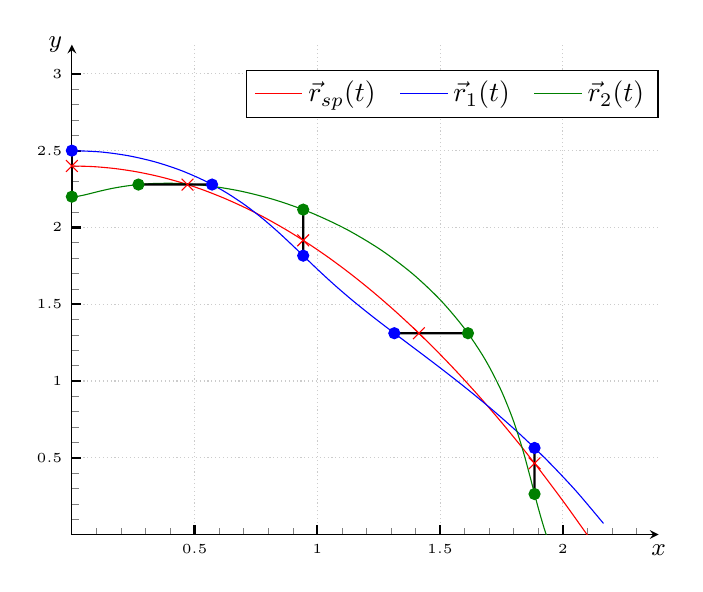
\begin{tikzpicture}
		\begin{axis}[
		    every minor tick/.append style={minor tick length=0.085cm},
		    every major tick/.append style={major tick length=0.12cm,thick,black},
			trig format plots=rad,
			width=257pt,
			height=222pt,
			axis lines=center,
			%	y axis line style={thick},
			tick align=outside,
			xmin=-0,xmax=2.39,ymin=-0,ymax=3.19,
			ticklabel style = {font=\tiny},
			tick align=inside,
			xlabel style={font=\small,below},
			ylabel style={font=\small,left},
			xtick distance=0.5,
			minor tick num=4,
			ytick distance=0.5,
			xlabel=$x$,
			ylabel=$y$,
			grid=major,
			grid style={thin,densely dotted,black!20},
			legend columns=3,
			legend style={at={(axis description cs:1,0.9)},anchor=east}],
			\addplot [domain=0:0.7,smooth, red]({3*x},{2.4-4.905*x^2});
			\addplot [domain=0:0.7,smooth, blue]({0.1*sin(10*x)+3*x},{2.4+0.1*cos(10*x)-4.905*x^2});
			\addplot [domain=0:0.7,smooth, Green]({-0.2*sin(10*x)+3*x},{2.4-0.2*cos(10*x)-4.905*x^2});
			\addplot [only marks,blue,mark=*] coordinates{(0,2.5) (0.571225, 2.27899) (0.942459, 1.81592) (1.31368, 1.31082) (1.88488, 0.563698)};\\
			\addplot [only marks,Green,mark=*] coordinates{(0,2.2) (0.271225, 2.27897) (0.942431, 2.11592) (1.61367, 1.31086) (1.88494, 0.263698)};
			\addplot [only marks,red,mark size=3pt, mark=x] coordinates{(0,2.4) (0.471225, 2.27898) (0.94245, 1.91592) (1.41368, 1.31083) (1.8849, 0.463698)};
			\draw[thick] (1.88488, 0.563698) -- (1.88494, 0.263698) 
				  (1.31368, 1.31086) -- (1.61367, 1.31086)
				  (0.942459, 1.81592) -- (0.942431, 2.11592)
				  (0.571225, 2.27899) -- (0.271225, 2.27897)
				  (0,2.2) -- (0,2.5) ;
			\legend{$\vec{r}_{sp}(t)$~~~,$\vec{r}_{1}(t)$~~~,$\vec{r}_{2}(t)$}
		\end{axis}
		\end{tikzpicture}
		\end{multicols}
		\item Im Schwerpunktsystem:
		\begin{flalign*}
			\vec{r}_{1,sp}(t) &= 0.1\ \vector{\sin(\omega t)\\ 0\\ \cos(\omega t)} \unit{m} &&\\
			\vec{r}_{2,sp}(t) &= -0.2\ \vector{\sin(\omega t)\\ 0\\ \cos(\omega t)} \unit{m} &&\\
		\end{flalign*}
		Im Laborsystem:\\
		\begin{flalign*}
			\vec{r}_1(t) &= \vec{r}_{sp}(t) + \vec{r}_{1,sp}(t) &&\\[2ex]
			&= \dl{\vector{0.1\sin(\omega t)\unit{m}\\ 0\\ 0.1\cos(\omega t)\unit{m} + 2.4\unit{\m}} + \vector{3\unit{\v}\\ 0\\ 0}t + \frac{1}{2} \vector{0\\ 0\\ -9.81\unit{\m\per\square\s}} t^2} &&\\[2ex]
			\vec{r}_2(t) &= \vec{r}_{sp}(t) + \vec{r}_{2,sp}(t) &&\\[2ex]
			&=  \dl{\vector{-0.2\sin(\omega t)\unit{m}\\ 0\\ -0.2\cos(\omega t)\unit{m} + 2.4\unit{\m}} + \vector{3\unit{\m\per\s}\\ 0\\ 0}t + \frac{1}{2} \vector{0\\ 0\\ -9.81\unit{\m\per\square\s}} t^2} &&\\
		\end{flalign*}
\end{enumerate}

\section*{140. International Space Station}
	\( R_E = 6.37 * 10^6 \unit{\m};\quad m = 4.55 * 10^5 \unit{\kg};\quad h = 3.3 * 10^5 \unit{\m} \)\\
\begin{enumerate}
	\item \( h = 0 \unit{m} \)
	\begin{flalign*}
		F_G &= mg \tfrac{1}{\left( 1 + \tfrac{h}{R_E} \right)^2} &&\\
		&= 4.55 * 10^5 \unit{\kg} * 9.81 \unit{\a} &&\\
		F_G &= \dl{4.46 * 10^6 \unit{kg.\a}} &&\\
	\end{flalign*}
	\item \( h = 3.3 * 10^5 \unit{\m} \)
	\begin{flalign*}
		F_G &= mg \tfrac{1}{\left( 1 + \tfrac{h}{R_E} \right)^2} &&\\
		&= 4.55 * 10^5 \unit{\kg} * 9.81 \unit{\a} \frac{1}{\left( 1 + \tfrac{3 * 10^5 \unit{\m}}{6.37 * 10^6 \unit{\m}} \right)} &&\\
		F_G &= \dl{4.03 * 10^6 \unit{kg.m/s^2}} &&\\[1.5ex]
		g(h) &= \tfrac{g}{\left( 1 + \tfrac{h}{R_E} \right)^2} &&\\
		g(3.3 * 10^5) &= \dl{8.87 \unit{m/s^2}} &&\\
	\end{flalign*}
	\newpage
	\centering\( v = r\omega;\quad a = \tfrac{v^2}{r} = r\omega^2;\quad r = R_E + h \)\\[1.5ex]
	\begin{minipage}{.3\textwidth}
	\item
	\begin{flalign*}
		\omega &= \sqrt{\tfrac{g(h)}{r}} &&\\
		&= \dl{1.2 * 10^{-3} \unit{s^{-1}}} &&
	\end{flalign*}	
	\end{minipage}
	\begin{minipage}{.3\textwidth}
	\item 
	\begin{flalign*}
		T &= \tfrac{2\pi}{\omega} &&\\
		&= \dl{5461.58 \unit{\s}} &&
	\end{flalign*}
	\end{minipage}
	\begin{minipage}{.3\textwidth}
	\item 
	\begin{flalign*}
		v &= r\omega &&\\
		&= \dl{7707.91 \unit{m/s}} &&
	\end{flalign*} 
	\end{minipage}
\end{enumerate}

\section*{152. Komprimierter Metallblock}
\begin{center}
	\begin{tabular}{ p{4cm} p{4cm} p{4cm} }
		$a = h = 0.2 \unit{\m}$ & $\Delta h = 1.3 * 10^{-6} \unit{\m}$ & $m = 500 \unit{\kg}$ \\[1.5ex]
		$V = 8 * 10^{-3} \unit{m^3}$ & $\Delta V = 3 * 10^{-7} \unit{\m^3}$ & $p = 2 * 10^6 \unit{kg/m.s^2} $
	\end{tabular}
\end{center}\vspace{1.5ex}
\begin{enumerate}
	\item \( p = K\ \tfrac{\Delta V}{V};\quad \tfrac{F}{A} = E\ \tfrac{\Delta h}{a} \)
	\begin{flalign*}
		K &= p\ \tfrac{V}{\Delta V} &&\\
		&= \dl{\tfrac{16}{3} * 10^{10} \unit{kg/m.s^2}}&&\\[1.5ex]
		E &= \tfrac{mga}{a^2 \Delta h} &&\\
		&= \dl{1.89 * 10^{10} \unit{kg/m.s^2}} &&
	\end{flalign*}
	\item \(\Delta a = \mu \Delta h;\quad K = \tfrac{E}{3(1-2\mu)} \)
	\begin{flalign*}
		K &= \tfrac{E}{3(1-2\mu)} &&\\
		\tfrac{3K}{E} &= \tfrac{1}{1-2\mu} &&\\
		\mu &= \tfrac{1}{2} - \tfrac{E}{6K} &&\\
		&= \dl{0.44} &&\\[2ex]
		\Delta a &= \mu\Delta h &&\\
		&= \dl{5.73 * 10^{-7} \unit{m}} &&
	\end{flalign*}
\end{enumerate}


\end{document}